\documentclass[12,french]{report}
\usepackage{geometry}
\geometry{vmargin=3cm, hmargin=3cm}
\usepackage[T1]{fontenc}
\usepackage[utf8]{inputenc}
\usepackage[french]{babel}
\usepackage{graphicx}
\usepackage{amsmath}
\usepackage{amssymb}
\usepackage{sectsty}
\usepackage{authblk}
\usepackage{algpseudocode}
\usepackage{algorithm}
\usepackage{xspace}
\usepackage{mathtools}
\usepackage{mathrsfs}
\usepackage{enumitem}
\usepackage{titlesec}
\usepackage{hyperref}
\usepackage{xcolor}
\usepackage[justification=centering]{caption}
\usepackage{float}
\usepackage{tabto}
\usepackage{algorithm}
\usepackage{algpseudocode}

\usepackage{listings}
\usepackage{cleveref}

\renewcommand{\lstlistingname}{Code}
%\renewcommand{\figurename}{Fig.}

\lstdefinestyle{chstyle}{%
backgroundcolor=\color{gray!12},
basicstyle=\ttfamily\small,
showstringspaces=false,
numbers=left}

%\AddThinSpaceBeforeFootnotes
%\FrenchFootnotes

\titleformat{\chapter}[hang]{\bf\Huge}{\thechapter.}{2pc}{}
\titlespacing*{\chapter}{10pt}{0pt}{40pt}[0pt]
\newcommand{\HRule}{\rule{\linewidth}{0.5mm}}

\providecommand{\keywords}[1]{\textbf{\textit{Keywords:}} #1}
\bibliographystyle{apalike}

\usepackage{hyperref}

\begin{document}
\hypersetup{pdfborder=0 0 0}

\begin{titlepage}

\begin{center}
	\vspace*{\stretch{1}}
	\textsc{{\LARGE Institut national des sciences appliquées de Rouen} \\ 			\vspace{6mm} {\Large INSA de Rouen}} \\
	\vspace{5mm}
	
\includegraphics[width=0.4\textwidth]{./Images/insa}\\[1.0 cm]

	\textsc{\Large Projet Info GM4 - Vague 1}\\[0.6cm]

	% Title
	\HRule \\[0.5cm]
	{ \Huge \bfseries Algorithme Min-Max}\\[0.2cm]
	\HRule \\[0.75cm]

	
\includegraphics[width=0.7\textwidth]{./Images/Page_de_garde}\\[0.9 cm]

	% Author and supervisor
	\begin{minipage}{0.4\textwidth}
		\begin{flushleft} \large
			\emph{Auteurs:}\\
			Thibaut \textsc{André-Gallis} \\
			{\small\href{mailto:thibaut.andregallis@insa-rouen.fr}{thibaut.andregallis@insa-rouen.fr}} \\
			Kévin \textsc{Gatel} \\
			{\small\href{mailto:kevin.gatel@insa-rouen.fr}{kevin.gatel@insa-				rouen.fr}}\\
			Chloé \textsc{Mechelinck} \\
			{\small\href{mailto:chloe.mechelinck@insa-rouen.fr}{chloe.mechelinck@insa-rouen.fr}}
		\end{flushleft}
	\end{minipage}
	\begin{minipage}{0.4\textwidth}
		\begin{flushright} \large
			\emph{Enseignants:} \\
			Nathalie \textsc{Chaignaud} \\
			{\small\href{mailto:nathalie.chaignaud@insa-rouen.fr}								{nathalie.chaignaud@insa-rouen.fr}}\\
		\end{flushright}
	\end{minipage}
	\vspace*{\stretch{1}}

	\vfill
	{\large 07 Décembre 2021}
\end{center}
\end{titlepage}

\tableofcontents

%\listoffigures

\renewcommand{\chaptername}{}

\chapter*{Introduction}

But du projet : \\

Afin de mettre en ½uvre les compétences acquises dans le codage en
langage objet, nous avons choisi le projet consistant à implémenter
l'algorithme Min-Max dans le cas d'un jeu de dames.

Nous avons donc réaliser des recherches pour comprendre ces concepts
et pouvoir les implémenter. Cela nous a aussi permis de travailler
en équipe avec des personnes différentes de nos précédents projets.

\chapter{L'algorithme}

\section{Explication de l'algorithme du Minimax }

L'algorithme minimax ou minmax est un algorithme s'appliquant dans
le cas d'un jeu (donc dans le cadre de la théorie des jeu) à deux
joueurs lorsqu'il s'agit d'un jeu à somme nulle. Son objectif est
de minimiser la perte maximum. Un jeu est à somme nulle si la somme
des gains et des pertes de tous les joueurs est égale à 0, c'est à
dire la perte de l'un est le gain de l'autre. Ce type de jeu répond
à plusieurs caractéristiques, démontrées notamment par le théorème
du minimax de Von Neumann, dès 1926 (présence de configurations d'équilibre,
existance de l'algorithme...).

Le principe est globalement assez simple. L'ordinateur passe en revue
tous les possibilités pour chaque pièce sur un nombre limité de coup,
créant ainsi un arbre des possibilités (dont nous parlerons d'avantage
dans la 4ème partie dans nos exemples). Ensuite chaque noeud se voit
affecter une valeur en fonction des bénéfices du joueur et de l'adversaire.
Le choix retenu sera la branche partant d'une feuille de cette arbre
jusqu'à la racine, indiquant ainsi le coup qui doit être réalisé. 

Un problème de mémoire se pose alors car chaque pièce peut se déplacer
à gauche ou à droite (sauf si une pièce la bloque ou si le plateau
de jeu ne continue pas) et cela sur un seul coup. Si on réalise plusieurs
coups (ce qui est nécessaire), l'arbre devient rapidement très vaste.
En pratique, on explore souvent, lorsque l'algorithme est optimisé
une partie seulement de cet arbre à l'aide de méthodes dites d'élagage.

\section{Explication de la méthode alpha-béta et de l'élagage}

L'élagage alpha-bêta ( ou ...) est une méthode grâce à laquelle on
va pouvoir réduire la taille de l'arbre en enlevant certaines branches
à l'aide de conditions choisies. Ainsi, on réduit le nombre de noeuds
évalués et donc le temps de calcul de la branche ``à choisir''.
Il s'agit d'une optimisation du minimax sans perdre des informations. 

Cet élagage repose sur le fait qu'il n'est pas nécessaire d'examiner
les sous arbres dont la configuration et le résultat ne permettra
pas une amélioration du gain. On évalue pas les noeuds (et leur sous-arbre)
dont la qualité (le gain, l'intérêt) sera inférieur à un noeud déjà
évalué. Pour cela on va d'ailleurs travailler sur l'arbre dans un
sens fixé, ici de gauche à droite. 


\chapter{Le jeu de Dame}

\section{Implémentation du jeu de Dames}

Nous avons tout d'abord fixé les règles que nous allions respecter,
les variantes sur un jeu aussi populaire que les dames étant nombreuses.

Les pions ne peuvent pas se déplacer en arrière ni manger en arrière. 

Il est obligatoire pour un pion de manger lorsqu'il peut.

Les dames peuvent manger en arrière et se déplacer dans les quatres
diagonales sur l'espace de plusieurs cases. 

Nous avons réalisé notre code en java, langage que nous maitrisions
d'avantage. Nous allons d'abord donc brièvement présenter les classes qui concerne le jeu de dame principalement :

\subsection{Case}

La classe Case représente tout simplement une case du plateau du jeu de Dame. Elle possède donc des coordonnées, une couleur, une pièce qui peut être vide et plusieurs booléens qui ont un rôle dans l'implémentation et la partie graphique du jeu.
  
\subsection{Coordonnées}

La classe Coordonnées possède deux entiers x,y qui représentent juste des coordonnées sur le plateau. Nous avons crée cette classe pour ne pas avoir à transporter deux variables à chaque fois.

\subsection{Couleur}

Cette classe sert juste à différencier la couleur d'une pièce ou d'une case

\subsection{Damier}

La classe Damier est la classe principale du jeu de Dame. Elle représente le plateau du jeu mais pas seulement. Il contient également le tableau des pièces du jeu, le tableau des cases du jeu, la taille du plateau ainsi que plusieurs booléen qui jouent un rôle dans les règles du jeu et son déroulement. Elle possède également la procédure d'affichage principale du jeu.

\subsection{Joueur}

La classe Joueur représente un joueur du jeu évidemment. Elle se décline en deux classes qui héritent de joueur ordi et humain. Elles ne servent qu'à différencier si le joueur est un ordinateur ou un utilisateur sur sa machine. On retrouve les procédure AJoue qui implémente un coup dans le jeu, ainsi que APerdu qui retourne si le joueur a perdu ou gagné la partie.

\subsection{Lanceur}

Cette classe constitue le Main de notre programme, il est possible d'y modifier certains paramètre de la partie manuellement, sinon nous utilisons une autre classe que nous allons voir pour laisser le joueur décider des règles.

\subsection{Menu}

La classe menu permet de laisser l'utilisateur choisir ses règles pour la partie. Elle consiste simplement en un menu à choix multiples que l'on récupère et que l'on transmet au main pour lancer la partie.

\subsection{Piece}

La classe pièce correspond à une pièce du jeu elle se décompose en deux classes qui héritent de celle-ci : Pion et Reine qui sont les deux différents types de pièces qu'on retrouve dans le jeu de dame. Dans le fonctionnement de notre jeu c'est au niveau de la pièce que l'on vérifie si elle peut être mangée, si elle peut manger une autre pièce ainsi qu'afficher les déplacements possibles de la pièce.

\subsection{Souris}

La classe souris est sert à récupérer les actions de la souris pour permettre au joueur d'utiliser une souris pour jouer au lieu du clavier. Elle permet de récupérer les coordonnées de la case sur laquelle le joueur clique. 

\subsection{TableauPiece}

La classe TableauPiece gère la liste des pièces du jeu d'un camp comme de l'autre.


\section{Implémentation de la partie Algorithme Min Max et ses améliorations}

Nous allons maintenant nous intéresser d'avantage à la partie IA du projet. Nous allons détailler les classes du programme qui joue un rôle dans l'IA basée sur un algorithme min-max ainsi que certaines procédures importantes.

\subsection{Arbre}

\begin{figure}[H]
	\center
	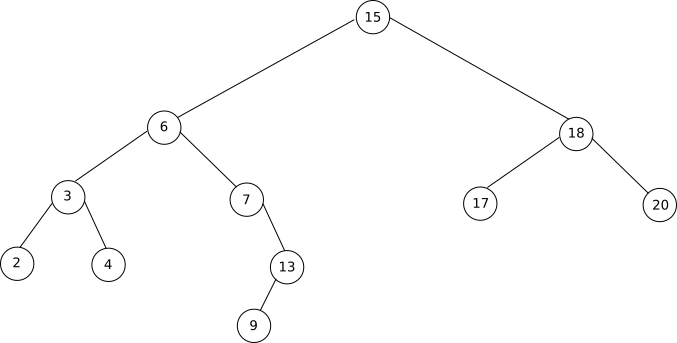
\includegraphics[width=0.8\textwidth]{./Images/arbre}
	\caption{Exemple d'un arbre quelconque}
\end{figure}\vspace{0.2cm}

La classe Arbre représente l'arbre sur lequel se base notre algorithme min-max. D'un point de vue informatique notre classe arbre est en fait la racine de l'arbre et on accède au reste de l'arbre grâce à la liste de successeurs qu'elle possède. C'est à dire que la classe arbre est le nœud tout en haut, nous allons maintenant définir ce qu'est un nœud dans notre cas de figure.

\subsection{NoeudDame}

La classe NoeudDame représente un nœud pour le jeu de dame dans le cadre de l'algorithme min-max. Elle implémente la classe abstraite Nœud. Nous l'avons donc défini comme un damier du jeu de dame. Un NoeudDame possède également une liste de NoeudDame qui lui succède et une valeur de profondeur permettant de savoir à quel profondeur de l'arbre il se situe. Cette classe possède également une des procédures les plus importante pour notre IA. Nous explorer l'Heuristique plus en détail car elle est essentielle pour le fonctionnement de l'IA.

\subsection{Coup}

La classe Coup représente un coup pour une pièce du jeu. Elle possède deux pièces celle au départ du coup et celle à la fin. Évidemment ce qui va changer entre deux sont les coordonnées de la pièce.

\subsection{Resultat\_minMax}

Cette classe a été crée pour exploiter le résultat retourné par notre méthode min-max. Elle n'a pas de signification particulière elle est juste une manière pratique de transporter les données dans ce cas. Pour résumer c'est une liste de coups à effectuer que nous renvoie notre algorithme min-max.

\subsection{Ordi}

La classe ordinateur implémente la classe joueur et représente un ordinateur dans le jeu. C'est dans cette classe que l'on retrouve l'algorithme min\_max que nous allons détailler ci-dessous. Tout d'abord nous allons écrire en pseudo-code la procédure min-max puis nous allons expliciter son fonctionnement.

\begin{algorithm}
	\caption{minMax(E : NoeudDame noeud; entier profondeurArbre)}
	\begin{algorithmic}
	\If{noeud est une feuille}
		\State retourner l'heuristique du nœud
	\EndIf
	\If{profondeur du fils est paire}
		\State valeur $\leftarrow$ -$\infty$
		\For{chaque fils de noeud}
			\State temporaire $\leftarrow$ minMax(fils,ProfondeurArbre,)
			\If{temporaire>valeur}
				\State valeur $\leftarrow$ temporaire
			\EndIf
		\EndFor
	\Else
		\State valeur $\leftarrow$ $\infty$
		\State temporaire $\leftarrow$ minMax(fils,ProfondeurArbre,)
		\If{temporaire<valeur}
			\State valeur $\leftarrow$ temporaire
		\EndIf
	\EndIf
	\end{algorithmic}
\end{algorithm}

\pagebreak

\underline{Explications minMax:}\\

L'algorithme minMax à partir d'un arbre dont les nœuds sont des damiers du jeu de dame doit ressortir le meilleur coup à jouer pour l'ordinateur.\\
On part de la racine qui représente le damier actuelle, chacun des nœuds fils d'un nœud représente une situation possible avec un coup d'écart avec le nœud père. La profondeur de l'arbre qu'on explore va avoir un lien direct avec la difficulté de l'ordinateur. Plus l'arbre est profond plus l'ordinateur fera son choix en fonction des conséquences à plus long termes. Autrement dit la profondeur de l'arbre correspond au nombre de coup d'avance avec lequel joue l'ordinateur. \\
L'algorithme consiste à évaluer les feuilles de l'arbre grâce à la fonction heuristique en leur donnant une valeur représentative de l'intérêt de la situation pour le joueur. Ensuite en fonction de si le niveau auquel on se situe  est paire ou impaire on remonte la valeur maximal ou minimal des fils au nœud père. à la fin on obtient le coup qui maximise l'intérêt pour l'ordinateur tout en minimisant l'intêret pour l'adversaire. Plus la profondeur de l'arbre va être grande plus on va pouvoir cela à long terme.\\
L'algortihme semble parfait et imbattable si on pousse la profondeur au maximum, cependant le coût de calcul et la consommation de mémoire est exponentielle et on arrive rapidement aux limites de l'ordinateur même pour le jeu de dame. Il existe donc certaines méthodes pour réduire le coût de calcul comme l'élagage alpha-béta que nous n'avons pas eu le temps de mettre en place.
L'autre faille importante est que la fonction heuristique elle ne peut être parfaite et résulte entièrement de l'interprétation humaine, mais on s'y est déjà intéressé précédemment.




%Le coeur de ce projet ce trouve dans cette partie. Nous avons d'abord
%fait un travail de recherches pour maîtriser ces concepts pour avancer
%ensuite plus rapidement et sereinement. Nous avons découpé notre travail
%comme présenté dans la partie 5 avec la modélisation UML.
%
%La fonction euristique est la pierre angulaire de cette partie, nous
%avons donc réfléchis et nous sommes renseignés sur les différentes
%positions (positions imprenables sur les côtés du plateau car les
%pions ne peuvent y être mangé ...) pour établir un ordre de priorité
%entre toutes et une valeur choisie sur une échelle de -5 pour la moins
%intéressante (position pour une dame de se faire manger) et 14 pour
%la plus intéressante (faire une dame). Cette échelle est encore sucesptible
%d'évoluer selon l'euristique que nous auront choisi puis si nous en
%testons plusieurs. Un seul déplacement peut en combiner plusieurs
%car un pion peut se mettre en position de manger et d'être manger
%aussi.
%
%L'action de manger étant obligatoire nous ne passont pas par la fonction
%euristique lorsque cette action se présente. C'est une des optimisations
%que nous comptons mettre en place.
%
%Nous avons aussi une fonction listecoups qui établit pour une composition
%donnée, une liste dynamique des positions possibles pour chaque pions.
%Cette liste est ensuite utilisée pour construire l'arbre vide sous
%forme de liste chainée puis de le remplir avec les valeurs des noeuds
%grâce à la fonction euristique.
%
%Enfin, nous avons la fonction parcoursminimax qui parcourt l'arbre
%avec l'algorithme minimax pour ressortir la branche la plus intéressante
%au niveau du gain.
%
%En bonus nous essayerons de rajouter la fonction élagage qui réalisera
%l'élagage détaillé dans les parties 3 et 4 juste avant la fonction
%parcoursminimax


\section{Application de la méthode à des exemples}

Pour mieux comprendre cette méthode et les différents cas possibles,
voici plusieurs exemples (simplifier car on a choisit de représenter
deux pions sur plusieurs coups en ayant attribué des valeurs aux noeuds).

\chapter{UML}

\section{diagramme de cas d'utilisation}

\begin{figure}[H]
	\center
	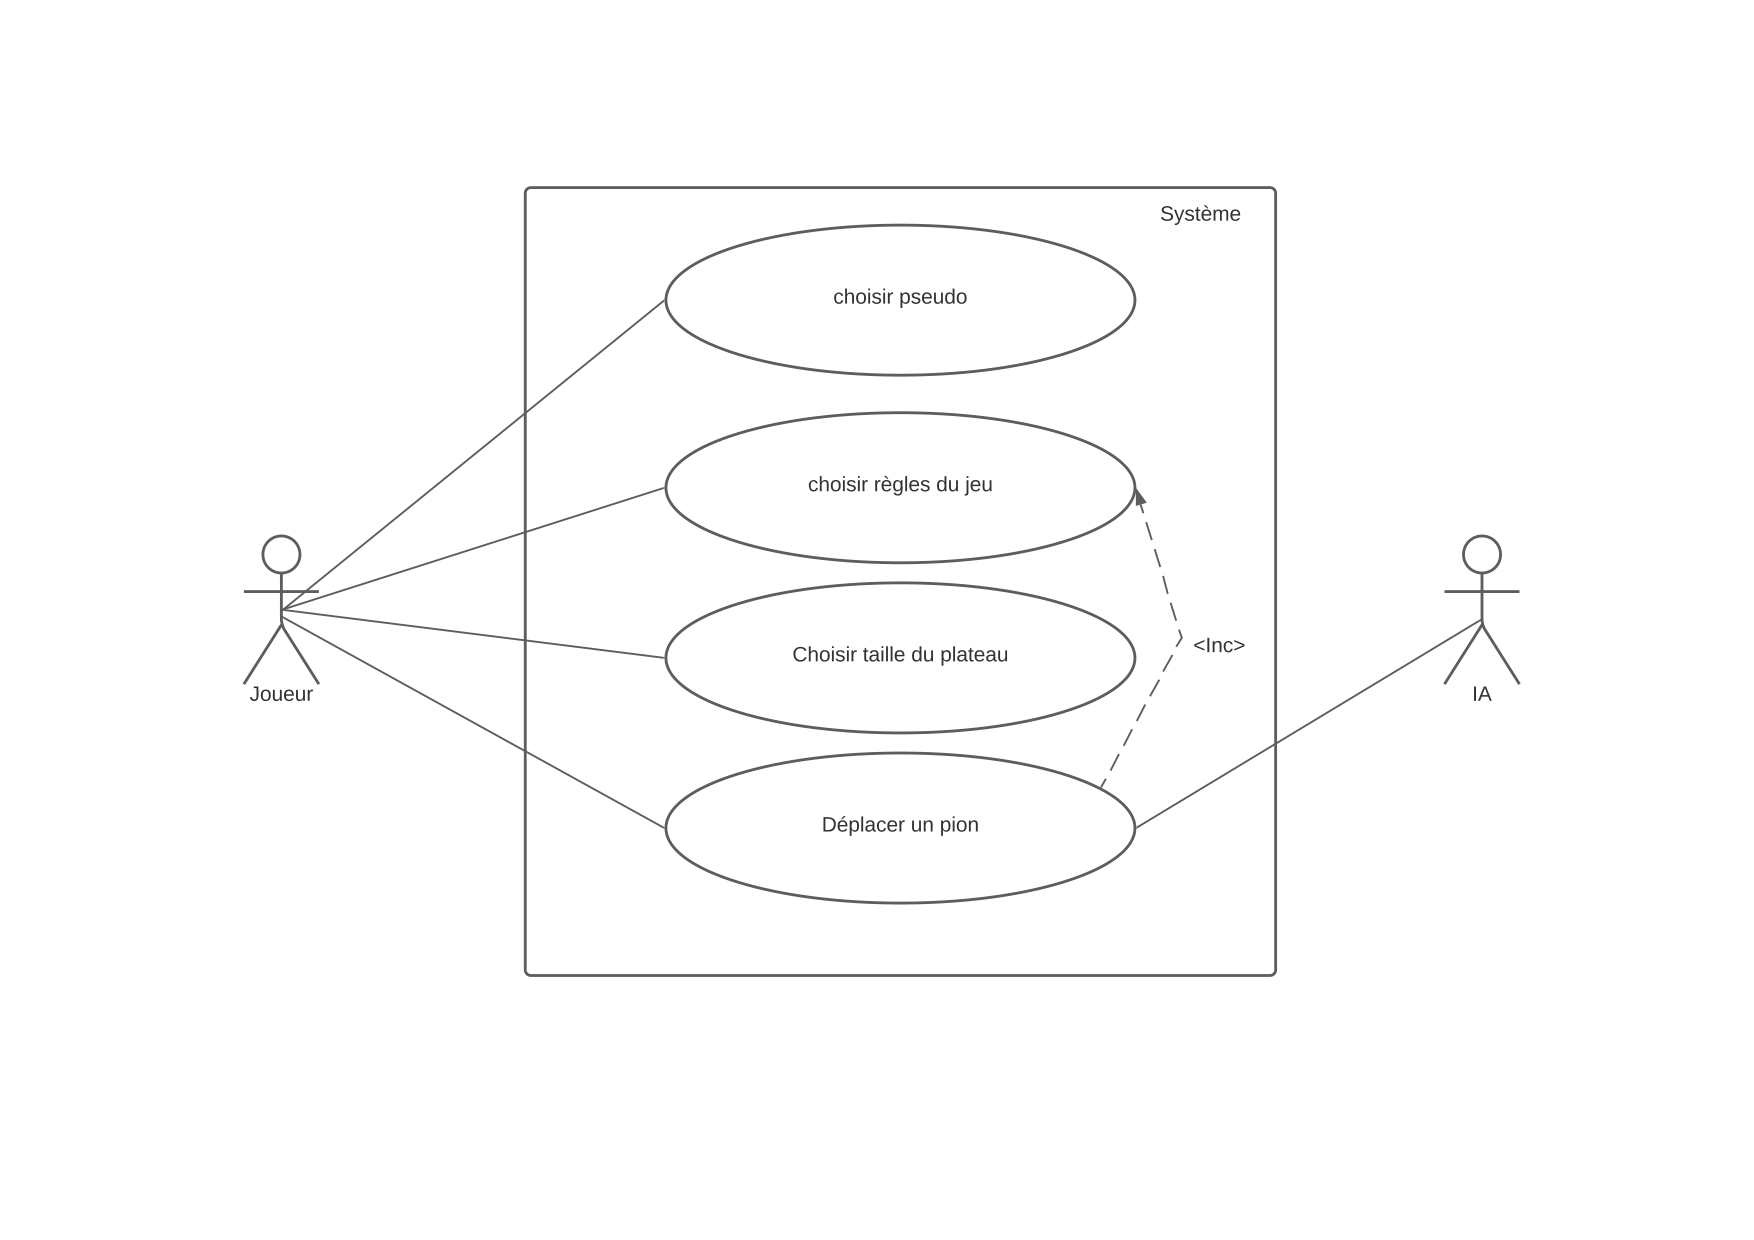
\includegraphics[width=1\textwidth]{./Images/Diagramme_use_case}
	\caption{Diagramme use case du jeu de dame}
\end{figure}\vspace{0.2cm}

L'utilisateur peut ainsi choisir de jouer à 2, de jouer contre l'ordinateur
ou afficher les règles, stockées dans un fichier texte extérieur.

\section{diagramme de séquences}

Nous avons réalisé plusieurs diagrammes de séquences pour détailler
la partie algorithme Min-max. Les voici:

\begin{figure}[H]
	\center
	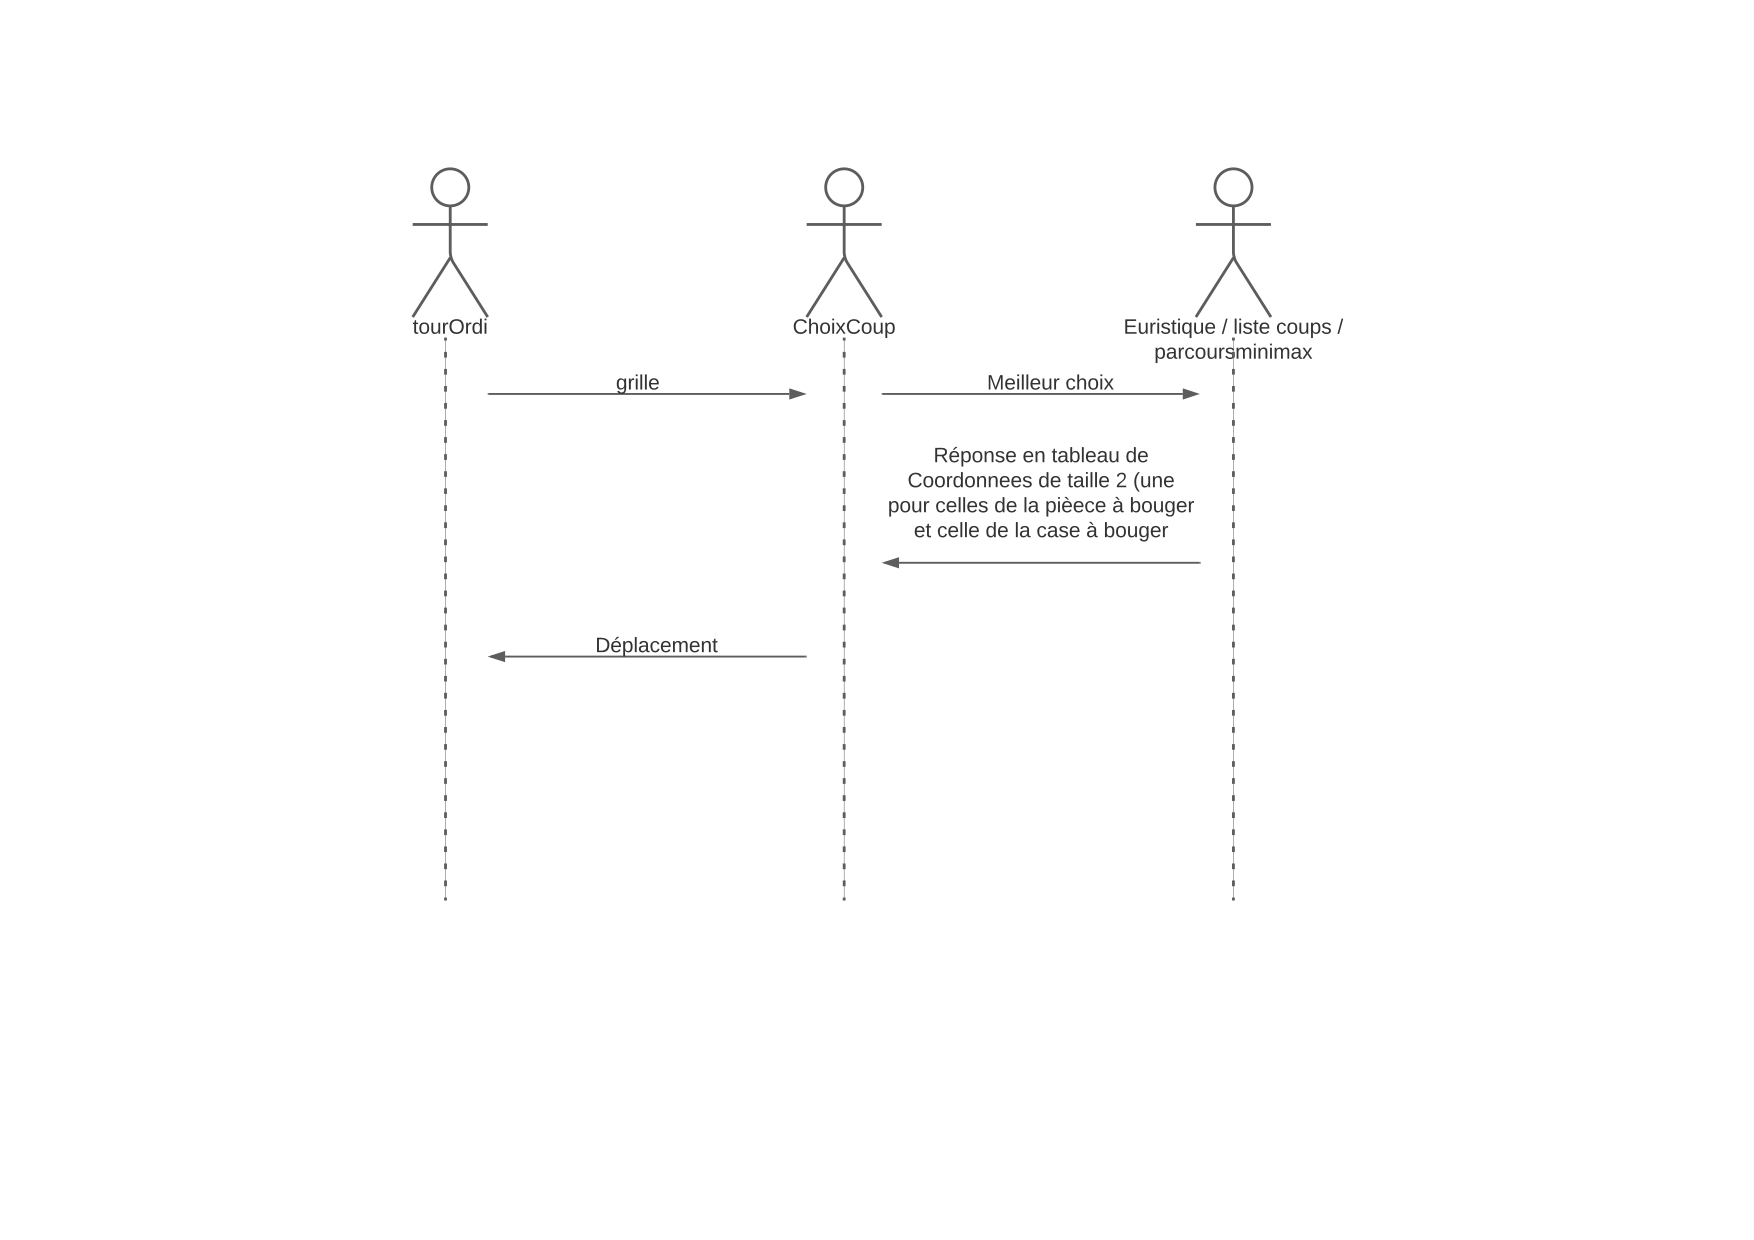
\includegraphics[width=0.8\textwidth]{./Images/Diagramme_de_sequence1}
	\caption{Diagramme de séquence choix coup ordi}
\end{figure}\vspace{0.2cm}

\begin{figure}[H]
	\center
	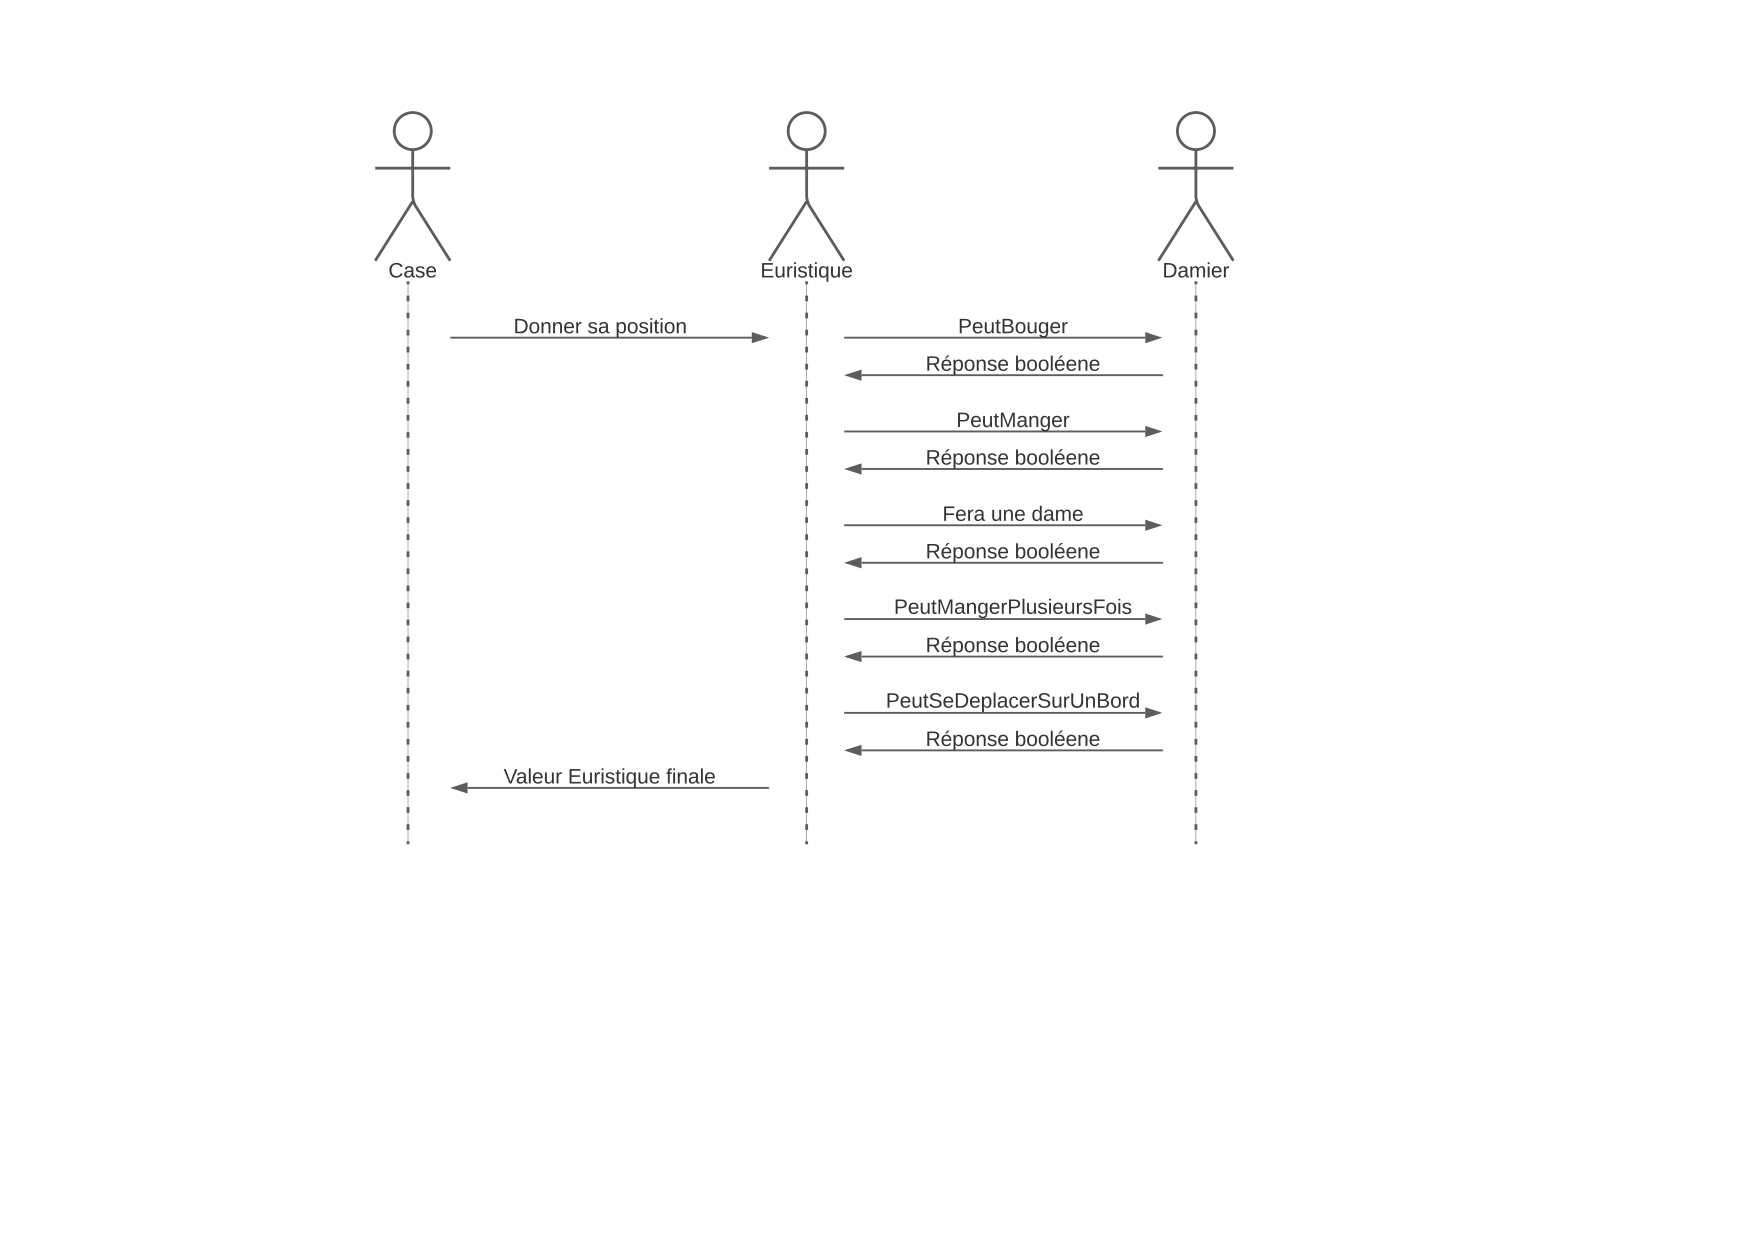
\includegraphics[width=0.8\textwidth]{./Images/Diagramme_de_sequence2}
	\caption{Diagramme de séquence heuristique}
\end{figure}\vspace{0.2cm}

\section{diagramme de classes}

\begin{figure}[H]
	\center
	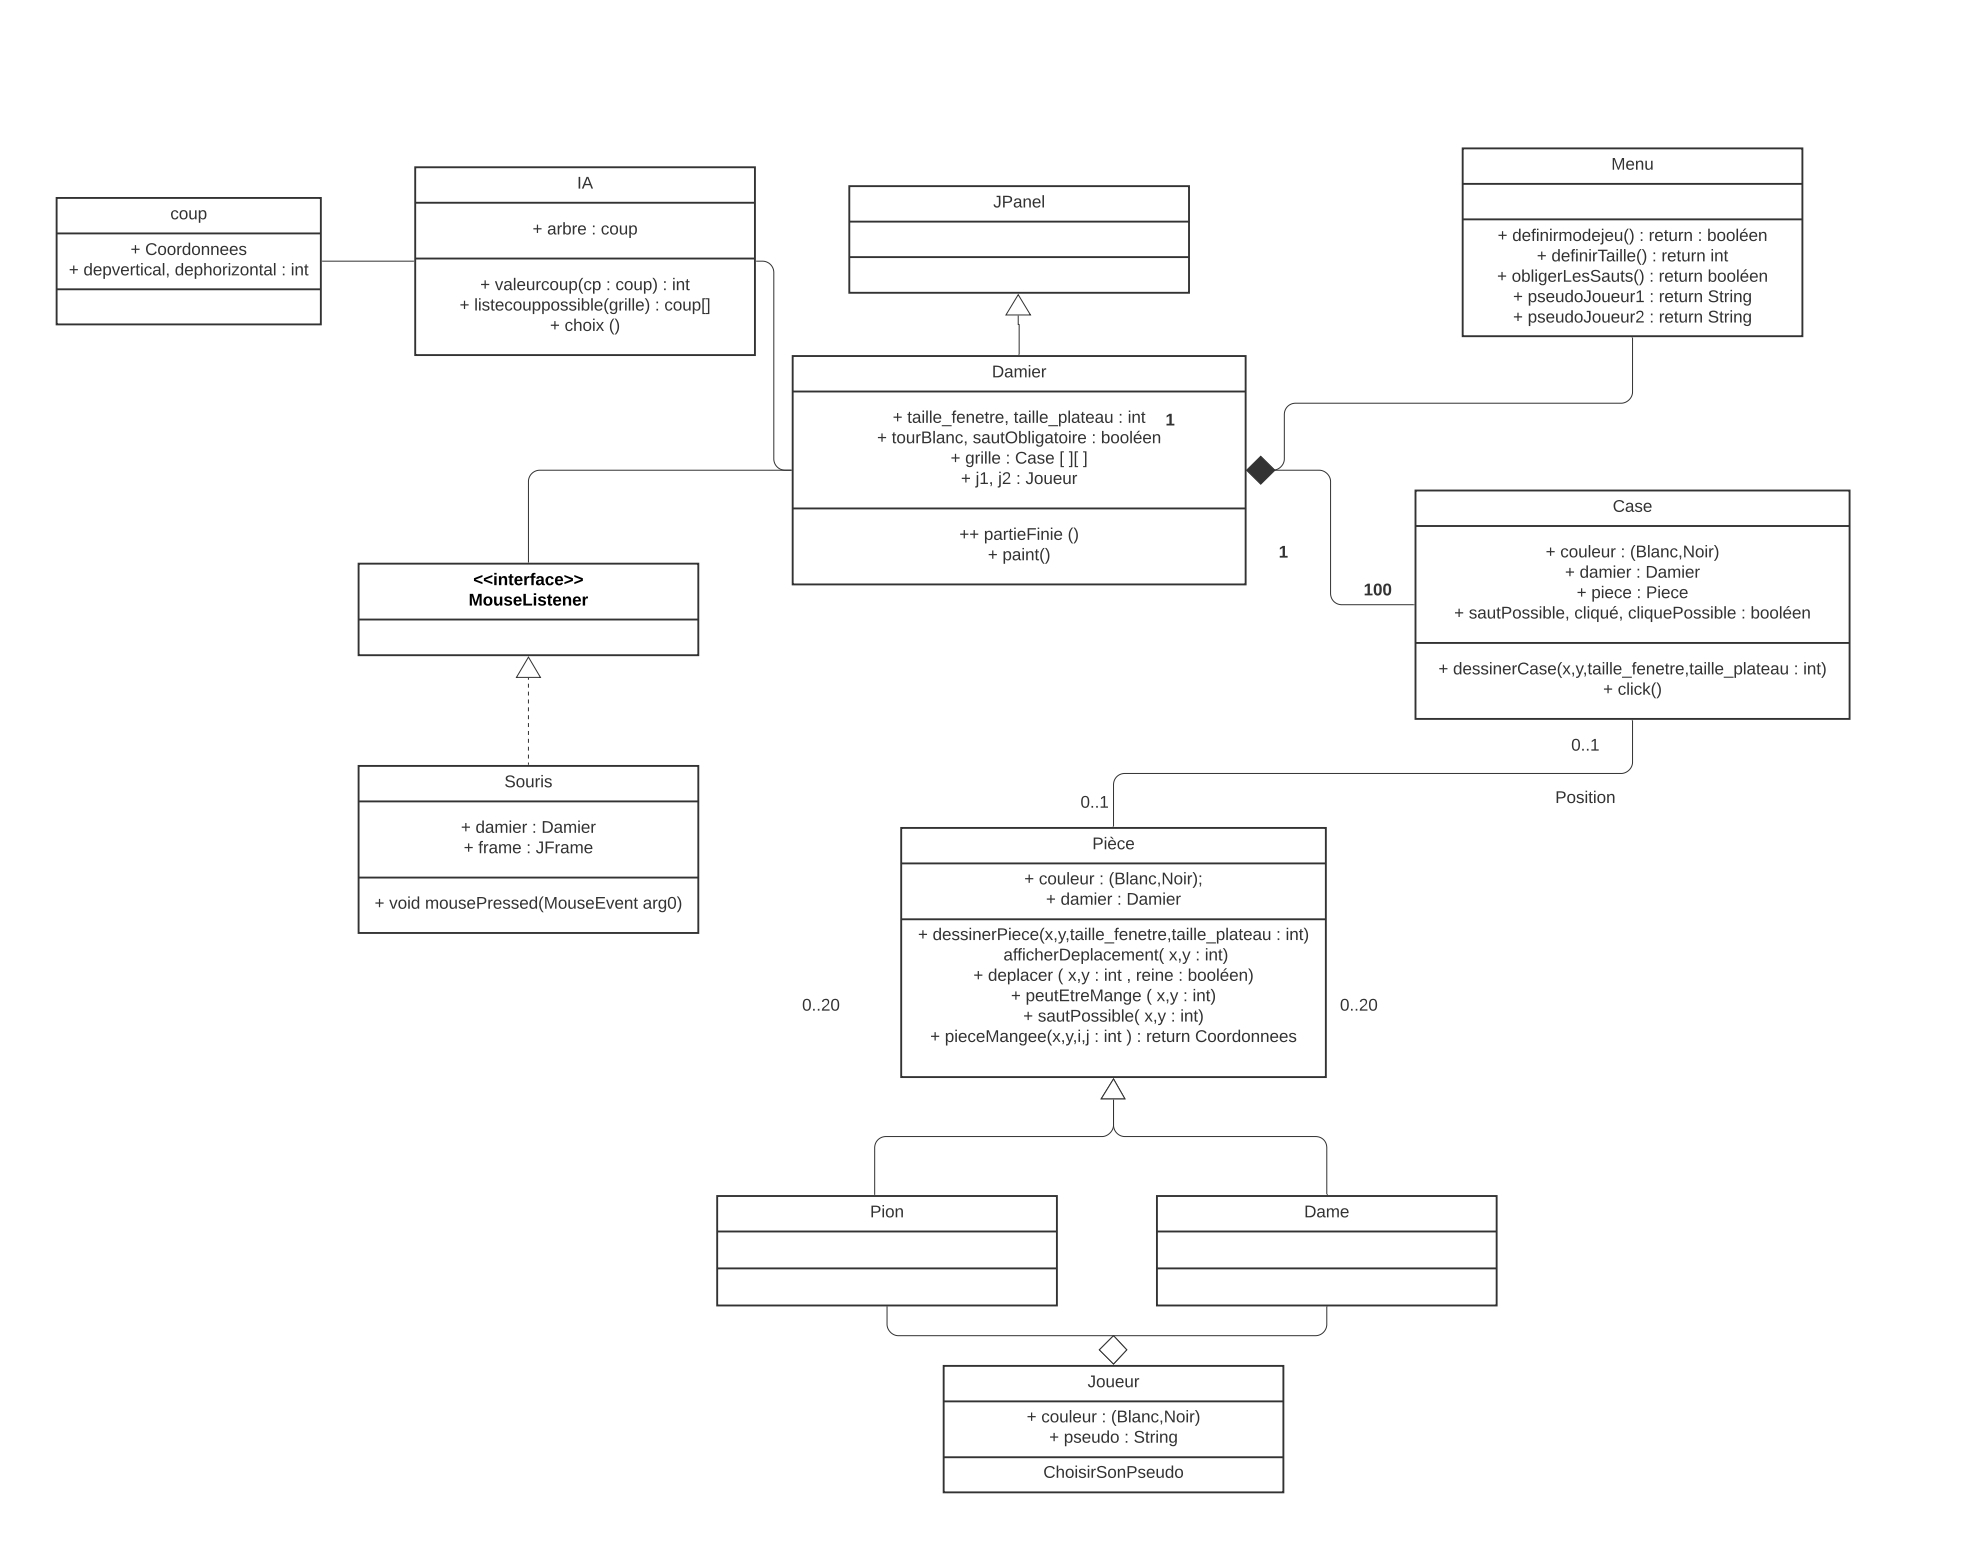
\includegraphics[width=1\textwidth]{./Images/Diagramme_classe}
	\caption{Diagramme des classes}
\end{figure}\vspace{0.2cm}

%\loadgame{\string"Diagramme UML\string"}\showboard


Voici le diagramme de classe de notre projet. Celui-ci est susceptible
d'évoluer jusqu'à la fin de notre code, il se sépare en deux parties:
la première pour l'implémentation du jeu de Dames la seconde pour
celle de l'algorithme Minimax.

Un certain nombre de fonction seront détaillées dans les parties suivantes.

\chapter*{Conclusion:}

Cette première partie nous a permis de nous renseigner sur la théorie
des jeux, les spécificité du jeu de Dames (les différents types de
positions des pions...). Nous avons aussi commencé à coder après avoir
réalisé nos diagrammes en essayant de rendre notre code le plus portable
possible, tout cela en travaillant en équipe à trois. Nous allons
poursuivre le codage de notre programme, tout en réalisant certaines
parties en pseudo-code d'abord car la fonction euristique est très
importante mais aussi assez importante.\\

\textbf{Pour aller plus loin :} \\

Comme dit précédemment nous ne sommes qu'au milieu de notre projet
et nous n'avons donc pas fini les fonctions de la partie implémentation
du mininmax.

Nous aimerions réaliser la fonction élagage, ainsi que plusieurs euristiques
que nous comparerions pour obtenir la meilleur (il s'agit de la difficulté
à laquelle sont confrontées les personnes ayant travaillé sur cet
algorithme etc: choisir la bonne euristique).

Si le temps qu'il nous reste nous le permet nous aimerions pouvoir
afficher à la demande du joueur, l'arbre des possiblités de sa composition
actuelle et la branche choisie. 

Nous voulons aussi réaliser un menu pour notre jeu avant le début
de la partie où l'on peut choisir de jouer à deux, seul contre l'ordinateur
ou bien d'afficher les règles.


\chapter*{Annexe}

\end{document}
